\begin{abstract}
%An abstract is a short (100 to 500 words), high-level summary of the entire document. 
%For this kind of report, you would start by introducing the concept that the report talks about and the goals of the work, followed by information about how the work was done and some summary of results.
The goal for the exercise was to get implement a 128-bit RSA encryption/decryption module for a FPGA. We opted to solve this problem by using a binary add implementation for dividing the modular exponentiation in a series of squaring and multiplications. \\
For the modular multiplication operations we implemented the Montgomery multiplication algorithm. This approach is also called for the Montgomery Exponentiation method. When simulating in Vivado the implementation met the timing constraints and used little area, but there are unfortunately no results from the FPGA as we had problems getting it running.


\begin{figure}[H]
\centering
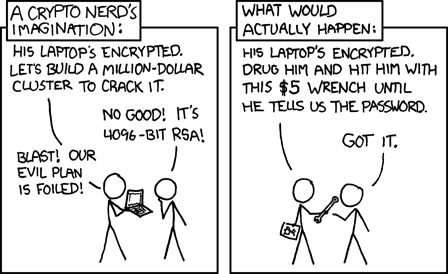
\includegraphics[width=0.7\textwidth]{images/security.png}
\caption{Mandatory XKCD: Security}
\label{fig:gamepad}
\end{figure}
\end{abstract}